
	\section{Strongest Stream Ciphers - eSTREAM Contest}
	
	eSTREAM was a crypto-contest held from 2004 till 2008 and aimed at discovering especially well-designed stream ciphers. eSTREAM came about due to another contest, NESSIE, which had no winners in the "Stream Ciphers" category because all of the ciphers had considerable vulnerabilities. Then, at the RSA Data Security Conference, it was argued whether stream ciphers can be considered obsolete if the Advanced Encryption Standard (AES) offers good solutions most of the time. However, there had been arguments that supported stream ciphers describing their advantages over block ciphers \cite{robshaw2008estream}:
	\begin{itemize}
		\setlength\itemsep{0.1em}
		\item Exceptionally high throughput in software.
		\item Exceptionaly low resource consumption in hardware.
	\end{itemize}
	To prove this, the European Network of Excellence for Cryptology (ECRYPT) launched the eStream project. It had three phases and featured different stream cipher designs in two Profiles \cite{robshaw2008estream}:
	\begin{itemize}
		\item[] Profile 1: Stream ciphers for software applications with high throughput.
		\item[] Profile 1A: Ciphers that satisfy Profile 1 with an associated authentification method.
		\item[] Profile 2: Stream ciphers for hardware applications with highly restricted resources (limited storage, gate count, or power consumption).
		\item[] Profile 2A: Ciphers that satisfy Profile 2 with an associated authentification method.
	\end{itemize}
	
	The following table pictures the initial requirements for the candidates:
	\begin{table}[h!]
		\centering
		\begin{tabular}{| c c c c|} 
			\hline
			& key length (bits) & IV length (bits) & tag length (bits) \\ [0.5ex] 
			\hline
			Profile 1 & 128 & 64 and 128 & - \\ 
			Profile 1A & 128 & 64 and 128 & 32, 64, 96 or 128 \\
			Profile 2 & 80 & 32 and 64 & - \\
			Profile 2A & 80 & 32 and 64 & 32 or 64 \\[1ex] 
			\hline
		\end{tabular}
		\label{table:Initial requirements for the candidates}
	\end{table}
	
	\textbf{Software-optimized ciphers} should significantly outperform the AES when used in a suitable stream cipher mode to justify stream cipher usage. It is important to point out that the contestants did not try to develop ciphers that were good at everything. The main focus was laid on raw encryption speed by large amounts of data after a single initialization. The security level was standard 128 bit, which matched contemporary applications very well.
	To evaluate all the contestants fairly, a special testing framework was introduced \cite{canniere2008estream}. It consisted of a collection of shell scripts and C-code and tested three aspects of every submitted cipher:
	\begin{enumerate}
		\item \emph{API compliance} checked if all the API requirements, like necessary interface, and key sizes are correct, if calls to the same function with the same parameters produce the same results or whether the encryption functions produce the same encrypted text from the same plaintext. 
		\item \emph{Correctness} of the code was verified by generating and comparing test vectors.
		\item \emph{Performance} was tested through the following criteria:
		\begin{itemize}
			\item \emph{Encryption rate} for long streams.
			\item\emph{Packet encryption} tested at which packet length a stream cipher would take the lead from a block cipher.
			\item \emph{Agility} tested the time spent switching from one session to another when encrypting many streams in parallel on one processor.
			\item \emph{Key and Initial Vector (IV) setup efficiency}.
		\end{itemize}
	\end{enumerate}
	
	\textbf{Hardware-optimized ciphers} should be significantly smaller and faster  than AES in a restricted environment in at least one significant aspect \cite{good2008asic}. These ciphers would be useful in, for example, sensor networks that are especially constrained in the number of logic gates or power. For this reason, the security level was chosen to be 80 bits.
	
	Like with any stream ciphers, an initialization vector (IV) and a secret key had to be used. For the 1A and 2A profiles, an authentification tag was also required.\\
	There were several evaluation criteria for each phase:
	\begin{itemize}
		\setlength\itemsep{0.1em}
		\item Security.
		\item Performance when compared to the AES in an appropriate mode.
		\item Performance, when compared to other submissions.
		\item Justification and supporting analysis simplicity and flexibility.
		\item Completeness and clarity of submission.
	\end{itemize}
	
	To go to the next phase a submission had to be notably better than AES.\\
	eSTREAM lasted four years and in 2008 a voting at SASC 2008 took place, where the finalists of the eSTREAM were evaluated on a scale from -5 to +5 and then the average was calculated. It is important to point out that this evaluation was not held by eSTREAM and should only be used for illustration. The following table demonstrates the results of the voting:
	\begin{table}[h!]
		\centering
		\begin{tabular}{|c c |c| c c|} 
			\hline 
			Rabbit & 2.80 & & Trivium & 4.35\\ 
			Salsa20 & 2.80 & & Grain v1 & 3.50\\
			SOSEMANUK & 1.20 & & MICKEY v2& 0.17\\
			HC-128 & 0.60 & & & \\[1ex]
			\hline
		\end{tabular}
		\label{table:eStream portfolio with SASC2008 evaluation}
	\end{table}
	
	This table also shows that the opinions about the hardware-optimized ciphers were more unified than the ones about the software-optimized ones.
	The ciphers that made it into the eStream portfolio can be divided into several categories \cite{jiao2020stream}:
	\begin{description}
		\item [ARX-based] (Addition/Rotation/XOR) are ciphers that only use module addition, interword rotation, and XOR to achieve required security strength. These operations are fast and easy to implement in software as well as they are immune to timing attacks because they run in constant time \cite{jiao2020stream}.
		Among the ciphers that made it into the eStream portfolio Rabbit and Salsa20 belong to ARX-based stream ciphers.
		\begin{figure}[h]
			
			\begin{subfigure}{0.5\textwidth}
				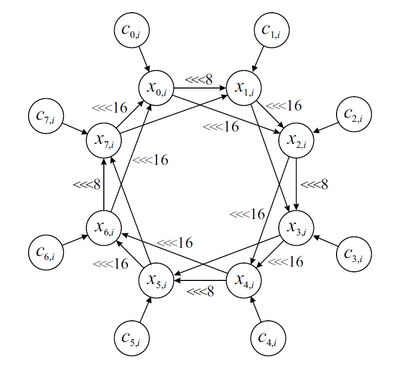
\includegraphics[width=1\textwidth]{img/rabbit.png} 
				\caption{Internal structure of the Rabbit cipher}
				\label{fig:rabbit}
			\end{subfigure}
			\begin{subfigure}{0.5\textwidth}
				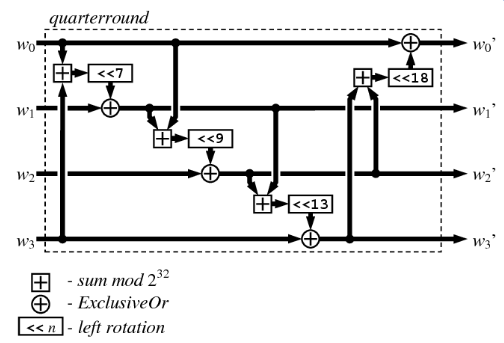
\includegraphics[width=1\textwidth]{img/salsa20.png} 
				\caption{Internal structure of the Salsa20/r ciphe}
				\label{fig:salsa20}
			\end{subfigure}
			
			\caption{ARX-based eStream finalists}
			\label{fig:arx}
		\end{figure}
		
		\emph{Rabbit} is a software-efficient, synchronous stream cipher that uses a 128-bit key and a 64-bit IV. A set of eight state registers, each 32-bit long and eight 32-bit counters are used to provide encryption based on ARX operations. Testing during the eSTREAM process confirmed that the Rabbit cipher was one of the most efficient software-oriented stream ciphers submitted \cite{boesgaard2008rabbit}.\\
		\emph{Salsa20/r} is a software-oriented cipher that supports keys of 128 bits and 256 bits. During its operation, the key, a 64-bit nonce (unique message number), a 64-bit counter, and four 32-bit constants are mapped to the 512-bit initial state. After r iterations of the Salsa20/r round function, the updated state is used as a 512-bit keystream output. Due to its implementation Salsa20 resembles a block cipher \cite{bernstein2008salsa20}.
		Although many attacks on Rabbit and Salsa20 have been proposed, as of 2015, none of them have been more successful than brute force attacks. 
		\item [NLFSR-based] stream ciphers take NLFSR as the basic components. It uses both the nonlinear feedback and the nonlinear output to provide good sequence properties and security \cite{jiao2020stream}. 
		Among the eStream finalists, Trivium and Grain v1 belong to NLFSR-based ciphers.
		
		\begin{figure}[h]
			
			\begin{subfigure}{0.5\textwidth}
				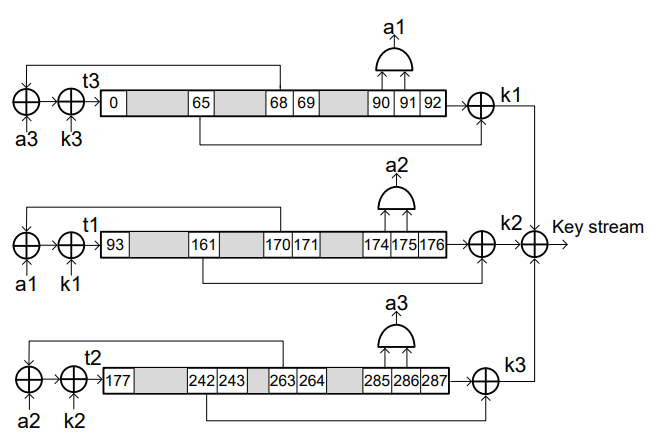
\includegraphics[width=1\textwidth]{img/trivium.png} 
				\caption{Internal structure of the Trivium cipher}
				\label{fig:trivium}
			\end{subfigure}
			\begin{subfigure}{0.5\textwidth}
				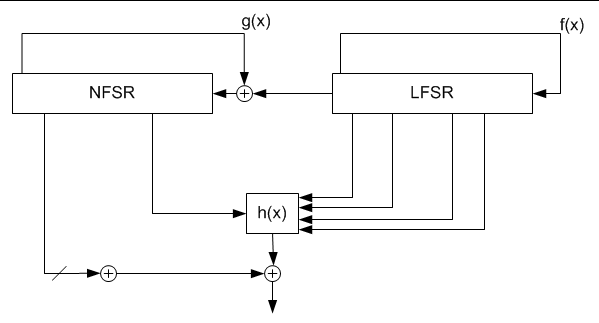
\includegraphics[width=1\textwidth]{img/grainv1.png} 
				\caption{Internal structure of the Grain v1 cipher}
				\label{fig:grainv1}
			\end{subfigure}
			
			\caption{NLFSR-based eStream finalists}
			\label{fig:NLFSR}
			
		\end{figure}
		
		\emph{Trivium} is a hardware-oriented stream cipher the main advantage of which is its simple design. It consists of three interconnected NLFSRs with feedback functions and linear or quadratic filter functions. It takes an 80-bit key and an 80-bit IV, and generates up to 264 keystream bits. It is important to note that Trivium was designed as an exercise, to explore how far a stream cipher can be simplified without sacrificing its security, speed or flexibility and still outperform AES \cite{canniere2008trivium}.\\
		\emph{Grain v1} combines the LFSR with the NLFSR, where LFSR provides good statistical characteristics and NLFSR adds nonlinear disturbance. A filter function is used to mix the state from both registers to further improve the security. It takes an 80-bit key and an 80-bit IV, using the LFSR and NLFSR each of 80-bit length, and a filter function of 5 variables and algebraic degree 3 \cite{hell2007grain}. A 2003 paper described a possible weakness in the cipher initialization \cite{kuccuk2006slide}. As of October 2006, no key recovery attacks better than brute force attacks are known against Grain v1.
		
		\item [LFSR-based] stream ciphers can be either bit-oriented (driven by one or more bit-unit LFSRs for a large cycle and good statistical properties, and usually combined with means of a filter, combiner, or clock control to realize the nonlinearly scrambling \cite{jiao2020stream}) or word-oriented (consists of the linear driver infinite field extension and a non-linear finite state machine (FSM), which can be regarded as a generalization of filter generators \cite{jiao2020stream}).
		
		\begin{figure}[h]
			
			\begin{subfigure}{0.5\textwidth}
				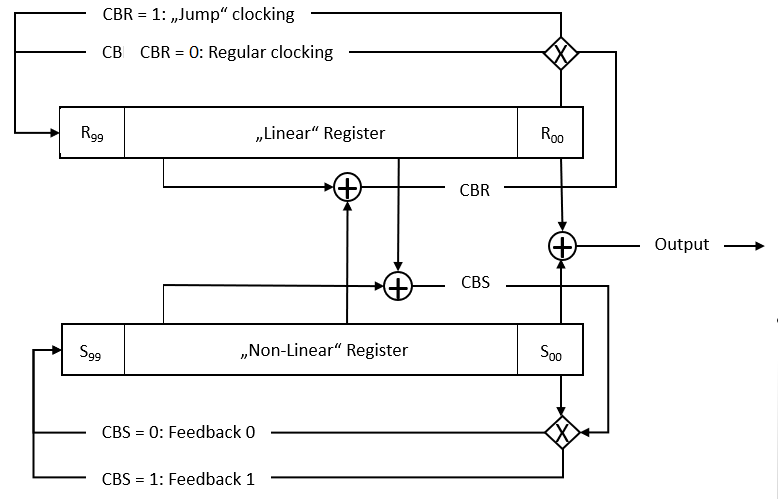
\includegraphics[width=1\textwidth]{img/mickeyv2.png} 
				\caption{Internal structure of the MICKEY v2 ciphe}
				\label{fig:mickeyv2}
			\end{subfigure}
			\begin{subfigure}{0.5\textwidth}
				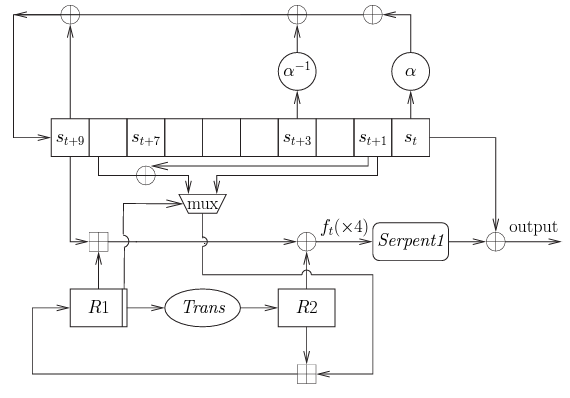
\includegraphics[width=1\textwidth]{img/SOSEMANUK.png} 
				\caption{Internal structure of the SOSEMANUK cipher}
				\label{fig:sosemanuk}
			\end{subfigure}
			
			\caption{LFSR-based eStream finalists}
			\label{fig:lfsr}
			
		\end{figure}
		
		
		\emph{Mickey v2} is a bit-oriented LFSR-based cipher. It uses irregular timing of shift registers, as well as new methods that provide a sufficiently large period and pseudo-randomness of the key sequence and resistance to attacks \cite{babbage2006stream}. As of 2013, a differential fault attack has been reported \cite{banik2015improved}.\\
		\emph{SOSEMANUK} is a word-oriented LFSR-based cipher influenced by the stream cipher SNOW and the block cipher SERPENT. Like the SNOW cipher, the SOSEMANUK algorithm uses two basic concepts: an LFSR and an FSM. The data obtained using the LFSR is fed to the input of the FSM, where it is non-linearly transformed. The four output values of the state machine are then table-swapped and XORed with the appropriate shift register values. The key schedule for the cipher is compiled using the Serpent24 primitive \cite{berbain2008sosemanuk}. Several attacks on SOSEMANUK have been published \cite{tsunoo2006evaluation} \cite{lee2008cryptanalysis}. However, none of the proposed attacks breaks the claimed 128-bit security of the cipher.
		
		\item [Random shuffled] stream ciphers achieve high efficiency of software implementation by employing randomly shuffled tables that shuffle a list to create random permutations, based on the RC4 cipher design. Since RC4 has got a number of applications in practice, it inspired subsequent designs of this type of structure, against which the state recovery attacks often require extremely high time complexity \cite{jiao2020stream}. 
		
		\begin{figure}[h]
			\centering
			\includegraphics[width=.5\textwidth]{img/hc-128.png}
			\caption{Internal structure of the HC-128 random shuffled cipher}
		\end{figure}
		
		A representative of this category in the eStream portfolio is the \emph{HC-128} cipher. Its internal state consists of two tables, each with 512 registers of 32 bits in length. At each step, one register of one of the tables is updated using a non-linear feedback function, while one 32-bit output is generated from the non-linear output filtering function. The cipher specifications state that 264 bits can be generated from each key/IV pair \cite{wu2008stream}.
		Despite the design's high profile, there have been no significant cryptanalytic advances against HC-128 since the publication of the eSTREAM portfolio.
		
	\end{description}
	
	\section{Trivium}
	
	In this section, we would like to show the functionality of a stream cipher on the example of the Trivium. This cipher was chosen for two reasons:
	\begin{enumerate}
		\setlength\itemsep{0.1em}
		\item Trivium has a very simple design, perfect for illustrative purposes.
		\item Trivium scored very highly at the SASC 2008 evaluation.
	\end{enumerate}
	
	\subsection{Functionality}
	
	Trivium consists of the following phases \cite{canniere2008trivium}:
	\begin{enumerate}
		\item \textbf{Initialization}
		\begin{itemize}
			\setlength\itemsep{0.1em}
			\item[-] IV: 80 bits.
			\item[-] Key: 80 bits.
			\item[-] Internal state: 288 bits ($s_1$, . . . , $s_{288}$). 
			\item[-] 4 * 288 = 1152 randomization cycles (after 1152 cycles a key stream is generated).
			\item[-] Key stream: N $\leq$ $2^{64}$ ($z_0$, ..., $z_n$), where N is the length of the plaintext.
		\end{itemize}
		At first, the  80-bit key (K) and an 80-bit initialization vector (IV) are loaded into the 288-bit internal state, all the remaining bits are set to 0s, except the last three, which are set to 1s. Then the bits in the register are randomized and rotated over 4 full cycles without generating keystream bits to improve randomization as well as dependency between the internal state, key and the initialization vector .
		The pseudo-code below shows the process in more detail:
		\vspace{0.5em}
		\\
		{\fontfamily{qcr}\selectfont
			($s_1$, $s_2$, ..., $s_93$) ← ($K_1$, ..., $K_{80}$, 0, ..., 0)\\
			($s_{94}$, $s_{95}$, ..., $s_{177}$) ← ($IV_1$, ..., $IV_{80}$, 0, ..., 0)\\
			($s_{178}$, $s_{279}$, ..., $s_{288}$) ← (0, ..., 0, 1, 1, 1)\\
			\textbf{for} i = 1 to 4 * 288 \textbf{do} \\
			\indent\hspace{1cm}$t_1$ ← $s_{66}$ $\oplus$ $s_{91}$ $\odot$ $s_{92}$ $\oplus$ $s_{93}$ $\oplus$ $s_{171}$\\
			\indent\hspace{1cm} $t_2$ ← $s_{162}$ $\oplus$ $s_{175}$ $\odot$ $s_{176}$ $\oplus$ $s_{177}$ $\oplus$ $s_{264}$\\
			\indent\hspace{1cm} $t_3$ ← $s_{243}$ $\oplus$ $s_{286}$ $\odot$ $s_{287}$ $\oplus$ $s_{288}$ $\oplus$ $s_{69}$\\
			\indent\hspace{1cm}($s_1$, $s_2$, ..., $s_{93}$) ← ($t_3$, $s_1$, ..., $s_{92}$)\\
			\indent\hspace{1cm}($s_{94}$, $s_{95}$, ..., $s_{177}$) ← ($t_1$, $s_{94}$, ..., $s_{176}$)\\
			\indent\hspace{1cm}($s_{178}$, $s_{279}$, ..., $s_{288}$) ← ($t_2$, $s_{178}$, ..., $s_{287}$)\\
			\textbf{end for}\\
		}
		\\
		The initialization procedure ensures that every bit of the initial state depends on every bit of the key and every bit of the initialization vector. This effect is achieved already after 2 full cycles (2*288 cycle executions). 2 more cycles are needed to complicate the bit relationships. For example, the first 128 bytes of the keystream, obtained from the null key and the initialization vector, have approximately the same number of 1s and 0s evenly distributed. Even with the simplest and identical keys, the Trivium algorithm produces a sequence of numbers that is close to random.
		\item \textbf{Stream generation}
		
		The keystream generation consists of an iterative process that extracts the values of 15 specific state bits and uses them both to update 3 bits of the state and to compute 1 bit of keystream $z_i$. The state bits are then rotated and the
		the process repeats itself until the requested N $\leq$ $2^{64}$ bits of keystream have been generated. The following pseudo-code describes the process in more detail:
		\vspace{0.5em}
		\\
		{\fontfamily{qcr}\selectfont
			\textbf{for} i = 1 \textbf{to} N \textbf{do}\\
			\indent\hspace{1cm}$t_1$ ← $s_{66}$ $\oplus$ $s_{93}$\\
			\indent\hspace{1cm}$t_2$ ← $s_{162}$ $\oplus$ $s_{177}$\\
			\indent\hspace{1cm}$t_3$ ← $s_{243}$ $\oplus$ $s_{288}$\\
			\indent\hspace{1cm}$z_i$ ← $t_1$ $\oplus$ $t_2$ $\oplus$ $t_3$\\
			\indent\hspace{1cm}$t_1$ ← $t_1$ $\oplus$ $s_{91}$ $\odot$ $s_{92}$ $\oplus$ $s_{171}$\\
			\indent\hspace{1cm}$t_2$ ← $t_2$ $\oplus$ $s_{175}$ $\odot$ $s_{176}$ $\oplus$ $s_{264}$\\
			\indent\hspace{1cm}$t_3$ ← $t_3$ $\oplus$ $s_{286}$ $\odot$ $s_{287}$ $\oplus$ $s_{69}$\\
			\indent\hspace{1cm}($s_1$, $s_2$, ..., $s_{93}$) ← ($t_3$, $s_1$, ..., $s_{92}$)\\
			\indent\hspace{1cm}($s_{94}$, $s_{95}$, ..., $s_{177}$) ← ($t_1$, $s_{94}$, ..., $s_{176}$)\\
			\indent\hspace{1cm}($s_{178}$, $s_{279}$, ..., $s_{288}$) ← ($t_2$, $s_{178}$, ..., $s_{287}$)\\
			\textbf{end for}
		}
	\end{enumerate}
	
	To better understand the algorithm, consider this example:
	\begin{enumerate}
		\setlength\itemsep{0.1em}
		\item We initialize a plaintext. For simplicity, it we will take an 'a'.\\
		{\fontfamily{qcr}\selectfont
			plainText = 0110 0001
		}
		
		
		\item We initialize a random initialization vector (IV) and a random key (K), 80 bits each.\\
		{\fontfamily{qcr}\selectfont
			\emph{K} = 0010 0101 1001 0101 1010 1011 0000 0011 0000 1101 0011\\
			\indent\hspace{1cm}1100 0010 0100 0001 0001 0111 0110 1110 1010
		}
		\vspace{0.5em}
		\\
		{\fontfamily{qcr}\selectfont
			\emph{IV} = 0111 0000 1100 0001 0101 0111 1100 0110 1101 0111 1110\\ 
			\indent\hspace{1.2cm}1000 1011 0111 0001 0000 1110 1110 0000 0111
		}
		
		\item For this example we initialize three shift registers, 288 bits in total. Where \emph{regA} is 93 bits long, \emph{regB} - 84 bits, and \emph{regC} is 111 bits long. The registers have to be loaded with the \emph{IV} and the \emph{K}. \\
		The first 80 bits of \emph{regA} are loaded with the \emph{K}, and the rest are 0. 
		\vspace{0.5em}
		\\
		{\fontfamily{qcr}\selectfont
			\emph{regA} = 0010 0101 1001 0101 1010 1011 0000 0011 0000 1101 0011 \\ 
			\indent\hspace{1.6cm}1100 0010 0100 0001 0001 0111 \textbf{0}110 1110 1\textbf{0}10 0\textbf{000}  0000\\
			\indent\hspace{1.6cm}00\textbf{00} \textbf{0}
		}
		\vspace{0.5em}
		\\
		The first 80 bits of \emph{regB} are loaded with \emph{IV}, the rest is 0. \\
		{\fontfamily{qcr}\selectfont
			\emph{regB} = 0111 0000 1100 0001 0101 0111 1100 0110 1101 0111 1110 \\ 
			\indent\hspace{1.6cm}1000 1011 0111 0001 0000 1\textbf{1}10 \textbf{1}110 0000 0111 0\textbf{000}
		}
		
		The last three bits of \emph{regC} are 1, the rest are 0.
		\vspace{0.5em}
		\\
		{\fontfamily{qcr}\selectfont
			\emph{regC} = 0000 0000 0000 0000 0000 0000 0000 0000 0000 0000 0000 \\ 
			\indent\hspace{1.6cm}1000 0000 0000 0000 0000 0\textbf{0}00 0000 0000 0000 0000 00\textbf{0}0 \\ 
			\indent\hspace{1.6cm}0000 0000 0000 0000 0000 \textbf{111}
		}
		\item As it is shown in the pseudo-code above, the bits are randomized with the help of XOR and AND operations, applied to the state register bits at the positions: 
		\vspace{0.5em}
		\\
		$regA_{66}$, $regA_{69}$, $regA_{91}$, $regA_{92}$, $regA_{93}$, \\
		$regB_{69}$, $regB_{78}$, $regB_{82}$, $regB_{83}$, $regB_{84}$, \\
		$regC_{66}$, $regC_{87}$, $regC_{109}$, $regC_{110}$, $regC_{111}$.
		\vspace{0.5em}
		\\
		This is repeated for four cycles.\\
		Operations with these chosen bits guarantee the longest period before bits start to repeat.\\
		After the randomization we get the following:
		
		{\fontfamily{qcr}\selectfont
			
			\emph{regA} = 1101 0111 1001 1001 0110 0111 0001 0010 1010 1000 0101 \\ 
			\indent\hspace{1.6cm}1000 1010 1011 1111 1100 0\textbf{1}10 \textbf{1}011 1001 0110 1100 1110 \\ 
			\indent\hspace{1.6cm}01\textbf{00} \textbf{1}
			
			\emph{regB} = 1101 1101 1101 0101 0111 0101 0011 1110 0001 0101 0011 \\ 
			\indent\hspace{1.6cm}1000 0011 0001 0111 0111 0011 \textbf{0}011 1001 1\textbf{1}10 1\textbf{100}
			
			\emph{regC} = 1111 0011 0000 0111 1001 0110 0101 0001 0100 0010 1011 \\ 
			\indent\hspace{1.6cm}1100 0000 0000 0011 1110 0\textbf{1}10 0001 1010 \textbf{1}000 1101 0111 \\
			\indent\hspace{1.6cm}0011 1010 1001 1000 100\textbf{0} \textbf{01}
		}
		\item Next step is the key generation. The procedure is similar to the Key and IV initialization, but now a key stream, the same length as the \emph{plainText}, is generated from the output variables:\\
		{\fontfamily{qcr}\selectfont
			$z_i$ ← $t_1$ $\oplus$ $t_2$ $\oplus$ $t_3$\\
			Where \\
			$t_1$ = $regA_{66}$ $\oplus$ $regA_{93}$\\
			$t_2$ = $regB_{69}$ $\oplus$ $regB_{84}$\\
			$t_3$ = $regC_{66}$ $\oplus$ $regC{111}$
		}
		\item \emph{$t_3$}, \emph{$t_1$}, \emph{$t_2$} are then added in the beginning of the \emph{regA}, \emph{regB}, \emph{regC} respectively, shifting this way bites. After eight iterations we have our \emph{keyStream}:\\
		{\fontfamily{qcr}\selectfont
			keyStream  = z = 0101 0111 = 'W'
		}
		\item Finally an encrypted text is generated by XORing corresponding bits from the key stream and from the plainText.\\
		{\fontfamily{qcr}\selectfont
			encryptedText = 0101 0111 $\oplus$ 0110 0001 = 0011 0110 = 6
		}
		\item By XORing the encrypted text with a keyStream, we can get our plain text back.\\
		{\fontfamily{qcr}\selectfont
			plainText = 0011 0110 $\oplus$ 0101 0111 = 0110 0001 = 'a'
		}
	\end{enumerate}
	
	\subsection{Security}
	According to the authors of the cipher \cite{canniere2008trivium}, it is harder to find \emph{correlations} between the internal state bits and the keystream in Trivium because as opposed to LFSR based ciphers, Trivium's state register is updated in a non-linear way, so it is harder for an attacker to recover the state.\\
	The non-linear nature of the cipher makes it nearly immune to the attacks that rely on determining its \emph{period} as well as \emph{algebraic attacks}. \emph{Resynchronization attacks} are avoided by cycling the state four times (step 4 in the example above) before producing any output. The authors name \emph{Guess and Determine attacks} as the ones of the most concern.\\
	In 2013 another team of researchers has shown that Trivium can be broken by a \emph{cube attack}, if the number of initialization rounds is reduced to 799 \cite{fouque2013improving}. 
	Only in 2020 \cite{potestad2020breaking} a not reduced version of Trivium was broken with the help of \emph{Experimental Attacks and Differential fault analysis (DFA)}. The idea is to inject faults into the Trivium clock cycle and get the faulty outputs. Then with the help of DFA the internal state is recovered through a comparison between correct and faulty outputs, after that, a specially designed Trivium version goes back and gets the initial key and the internal state. According to the authors, 100\% of keys have been recovered using this method.
	
	\section{Conclusion}
	In this paper, we have shown the principles, functionality, and mathematical basis of stream ciphers as well as evaluated their security. It is easy to notice that stream ciphers are a huge family united by the idea of streams of random numbers. And continuing the thought of John von Neumann, "...no such thing as a random number - there are only methods to produce random numbers." \cite[p.~36]{vonNeumann1951} we see that the variety of stream cipher designs is built on a pseudo-random flow of digits, which is just good enough to make things difficult for an attacker. Although all stream ciphers have an LFSR in them, it would be very insecure to use only an LFSR to create a random digit stream. LFSRs are not cryptographically secure because they are easy to reverse engineer. That is why stream ciphers usually have a non-linear part to improve security.\\
	As a result of our research, the following advantages of stream ciphers over block ciphers can be defined:
	\begin{enumerate}
		\setlength\itemsep{0.1em}
		\item Due to bit-by-bit operations, stream ciphers are more efficient and faster than block ciphers.
		\item They are better suited for environments with limited resources. 
		\item If there’s an error in one symbol, it’ll be less likely to affect the next.
		\item Easy to implement in hardware, using Flip-Flops and gates.
	\end{enumerate}
	The main disadvantages of stream ciphers, however, are:
	\begin{enumerate}
		\setlength\itemsep{0.1em}
		\item Due to looping in LFSRs, stream ciphers are not very software efficient.
		\item Stream ciphers are very vulnerable to bit-flipping and code reuse attacks because of their bit-by-bit approach. 
		\item Because stream ciphers work not with blocks, but with bits, an adversary can change a strategically chosen bit in the encrypted text to change the decrypted one.
	\end{enumerate}
	
	Stream ciphers are usually used where the amount of data is unknown or may be continuous, for example in wireless networking, or in the military. Nowadays the most common stream cipher used is ChaCha, which is based on Salsa20 we mentioned earlier, and its variations. \\
	Although stream ciphers are not especially widely used, it has been shown that they have their own niche, where they have considerable advantages over block ciphers and therefore more research should be put into this type of ciphers.
	\clearpage